
 \newpage
\section{SPI out}
\todo{JOHAN - FIX references further down this chapter}\\
This module is responsible for correctly outputtig data from the adder.


\subsubsection{Shift register}
The output consist of four sums, each containing 16 sum bits plus one carry output bit. This makes a total of 68 bits. To implement this we use a 68 bit shift register where each cell in the register contains one D flip-flop and one multiplexer. The multiplexer is used to switch between shifting and parallel load of the D flip-flop. In figure \ref{mux_dff} the schematic of a cell can be seen. 

\begin{figure}[H]
\centering
\captionsetup{justification=centering}
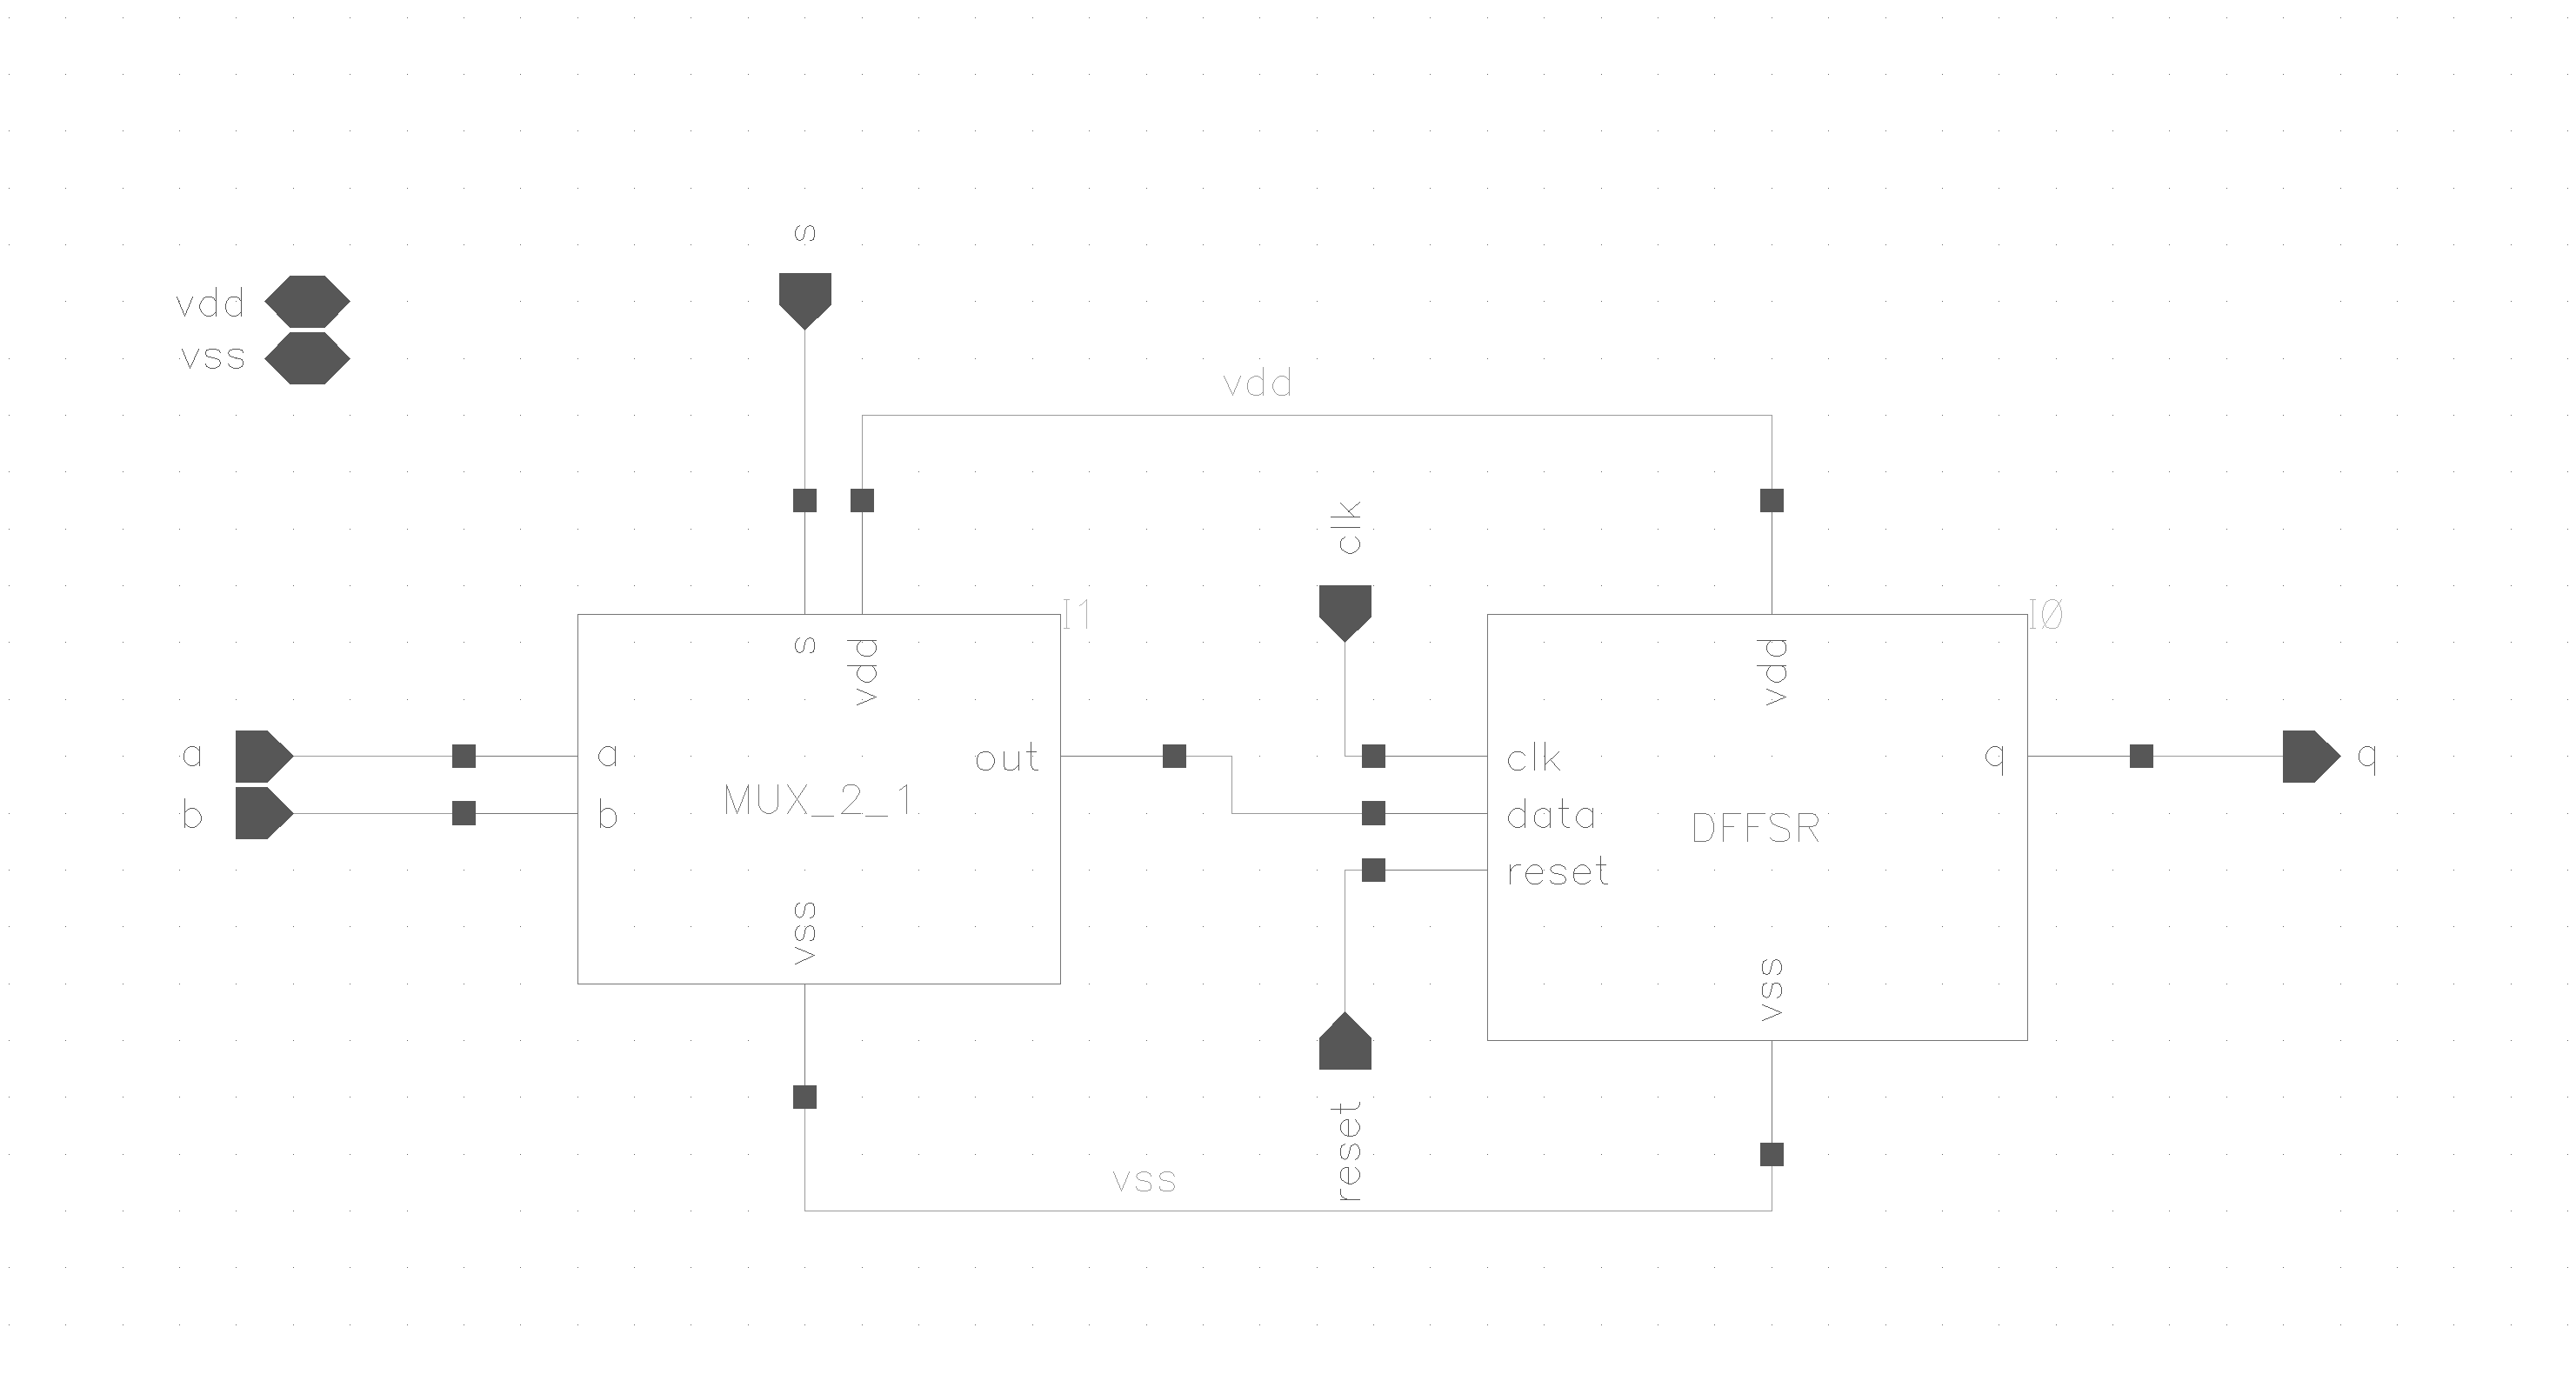
\includegraphics[scale=0.2]{../figures/mux_dffsr.png}
\caption{Shift register cell}
\label{mux_dff}
\end{figure}

\raggedright The spi enable signal is directly connected to the control signal of the multiplexer so that when spi enable is low, the input value to the D flip-flop is taken from the previous cell. 
 


\newpage

\subsubsection{Control logic}
The control logic is needed to load the long shift register with the correct data. \\
As the adder is built in such a way that it executes all the four additions as fast as it can after the spi enable signal goes high, the output from one addition will only be available for one system clock cycle. This means that we need to quickly grab the data and put it in the correct place.\\ 
Our implementation uses a pulse generator, a 2-bit counter, a decoder to select what 17-bit part of the shift register to load, and some multiplexers to select if to clock the register on the spi clock or on the enable signals from the decoder. The pulse generator is triggered by the spi enable signal and creates a pulse that is four system clock cycles long. This to only allow the counter to increment four times, and also to clip the pulse from the last decoder output. As can be seen in \ref{spi_out1} the last output of the decoder is also feeded back to the enable of the counter through an inverter. This prevents a possible glitch that is generated when the counter starts over. The glitch would reload the section of the shift register containing the first sum. \\

\begin{figure}[H]
\centering
\captionsetup{justification=centering}
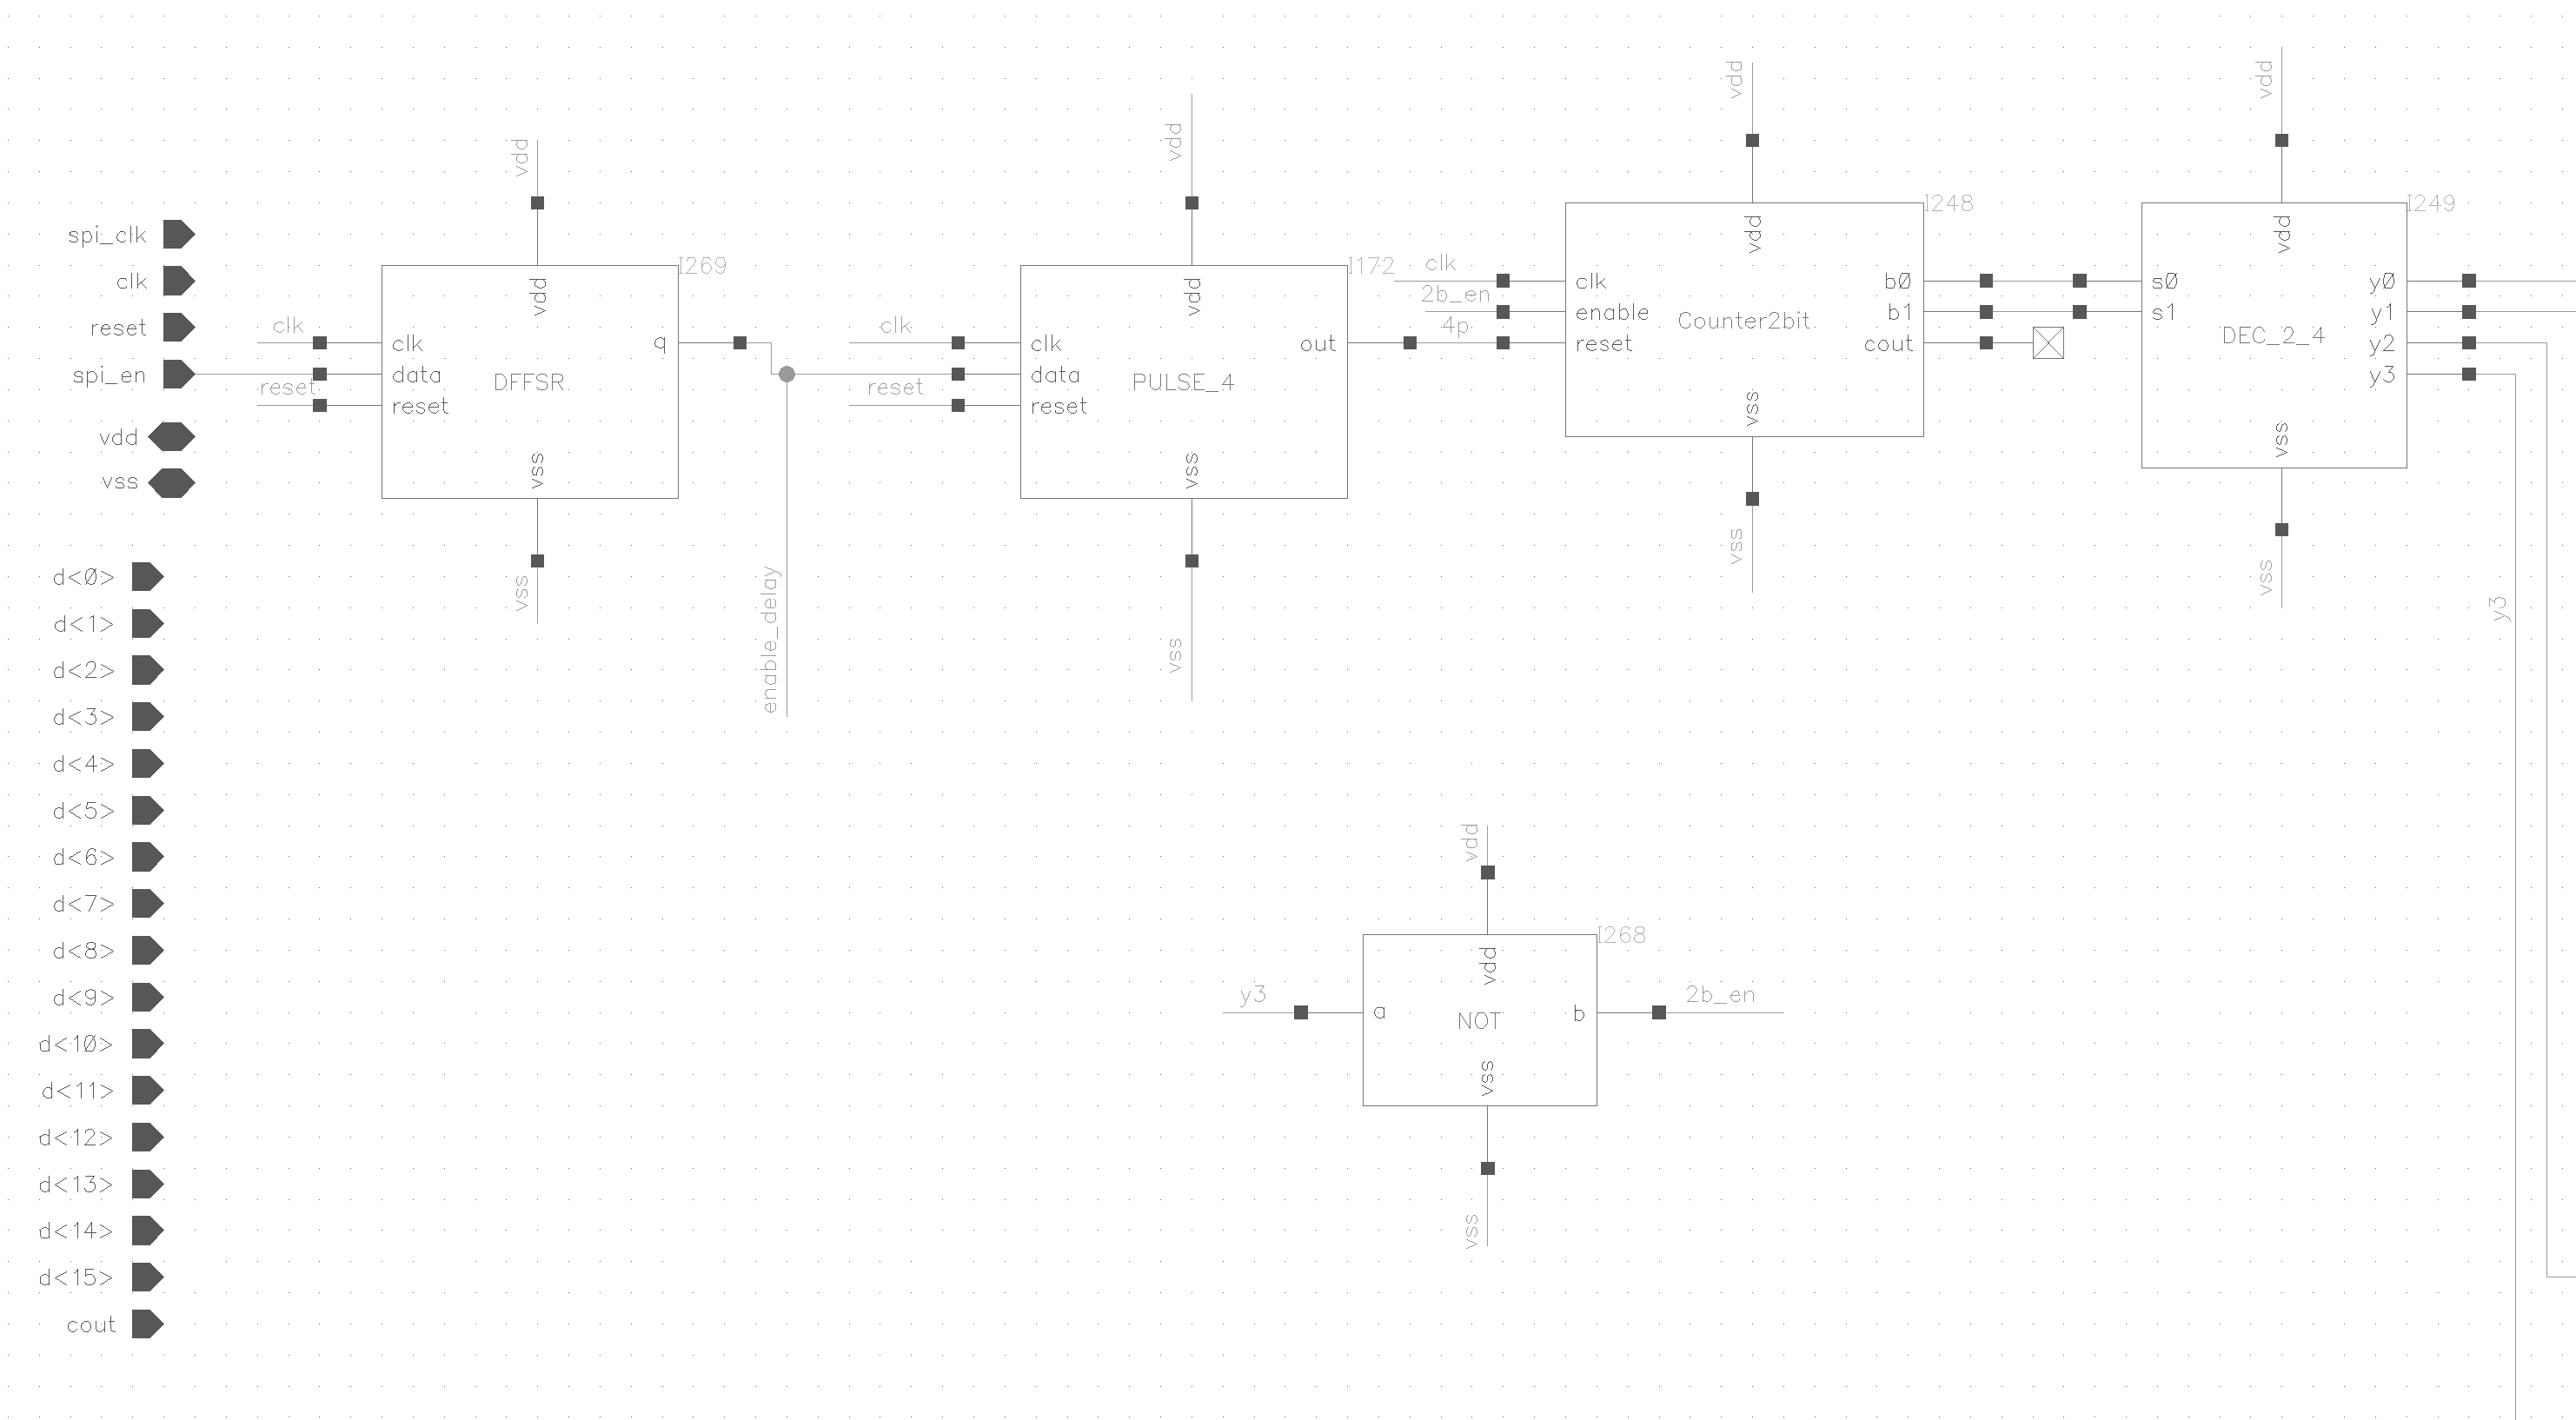
\includegraphics[scale=0.18]{../figures/spi_out1.png}
\caption{Control logic for spi output, first half}
\label{spi_out1}
\end{figure}

\newpage
\raggedright As can be seen to the right in figure \ref{spi_out2}, there are four enable signals: E1, E2, E3, E4. Each one of those signal enables a specific part of the shift register. If spi enable is low, all of the signals would be equal to the spi clock so that data can be shifted out. Otherwise, if the spi enable signal is high and, for example, E1 is high, the 17-bit part of the shift register corresponding to the sum of addition 1 would be loaded with the output from the adder.
\begin{figure}[H]
\centering
\captionsetup{justification=centering}
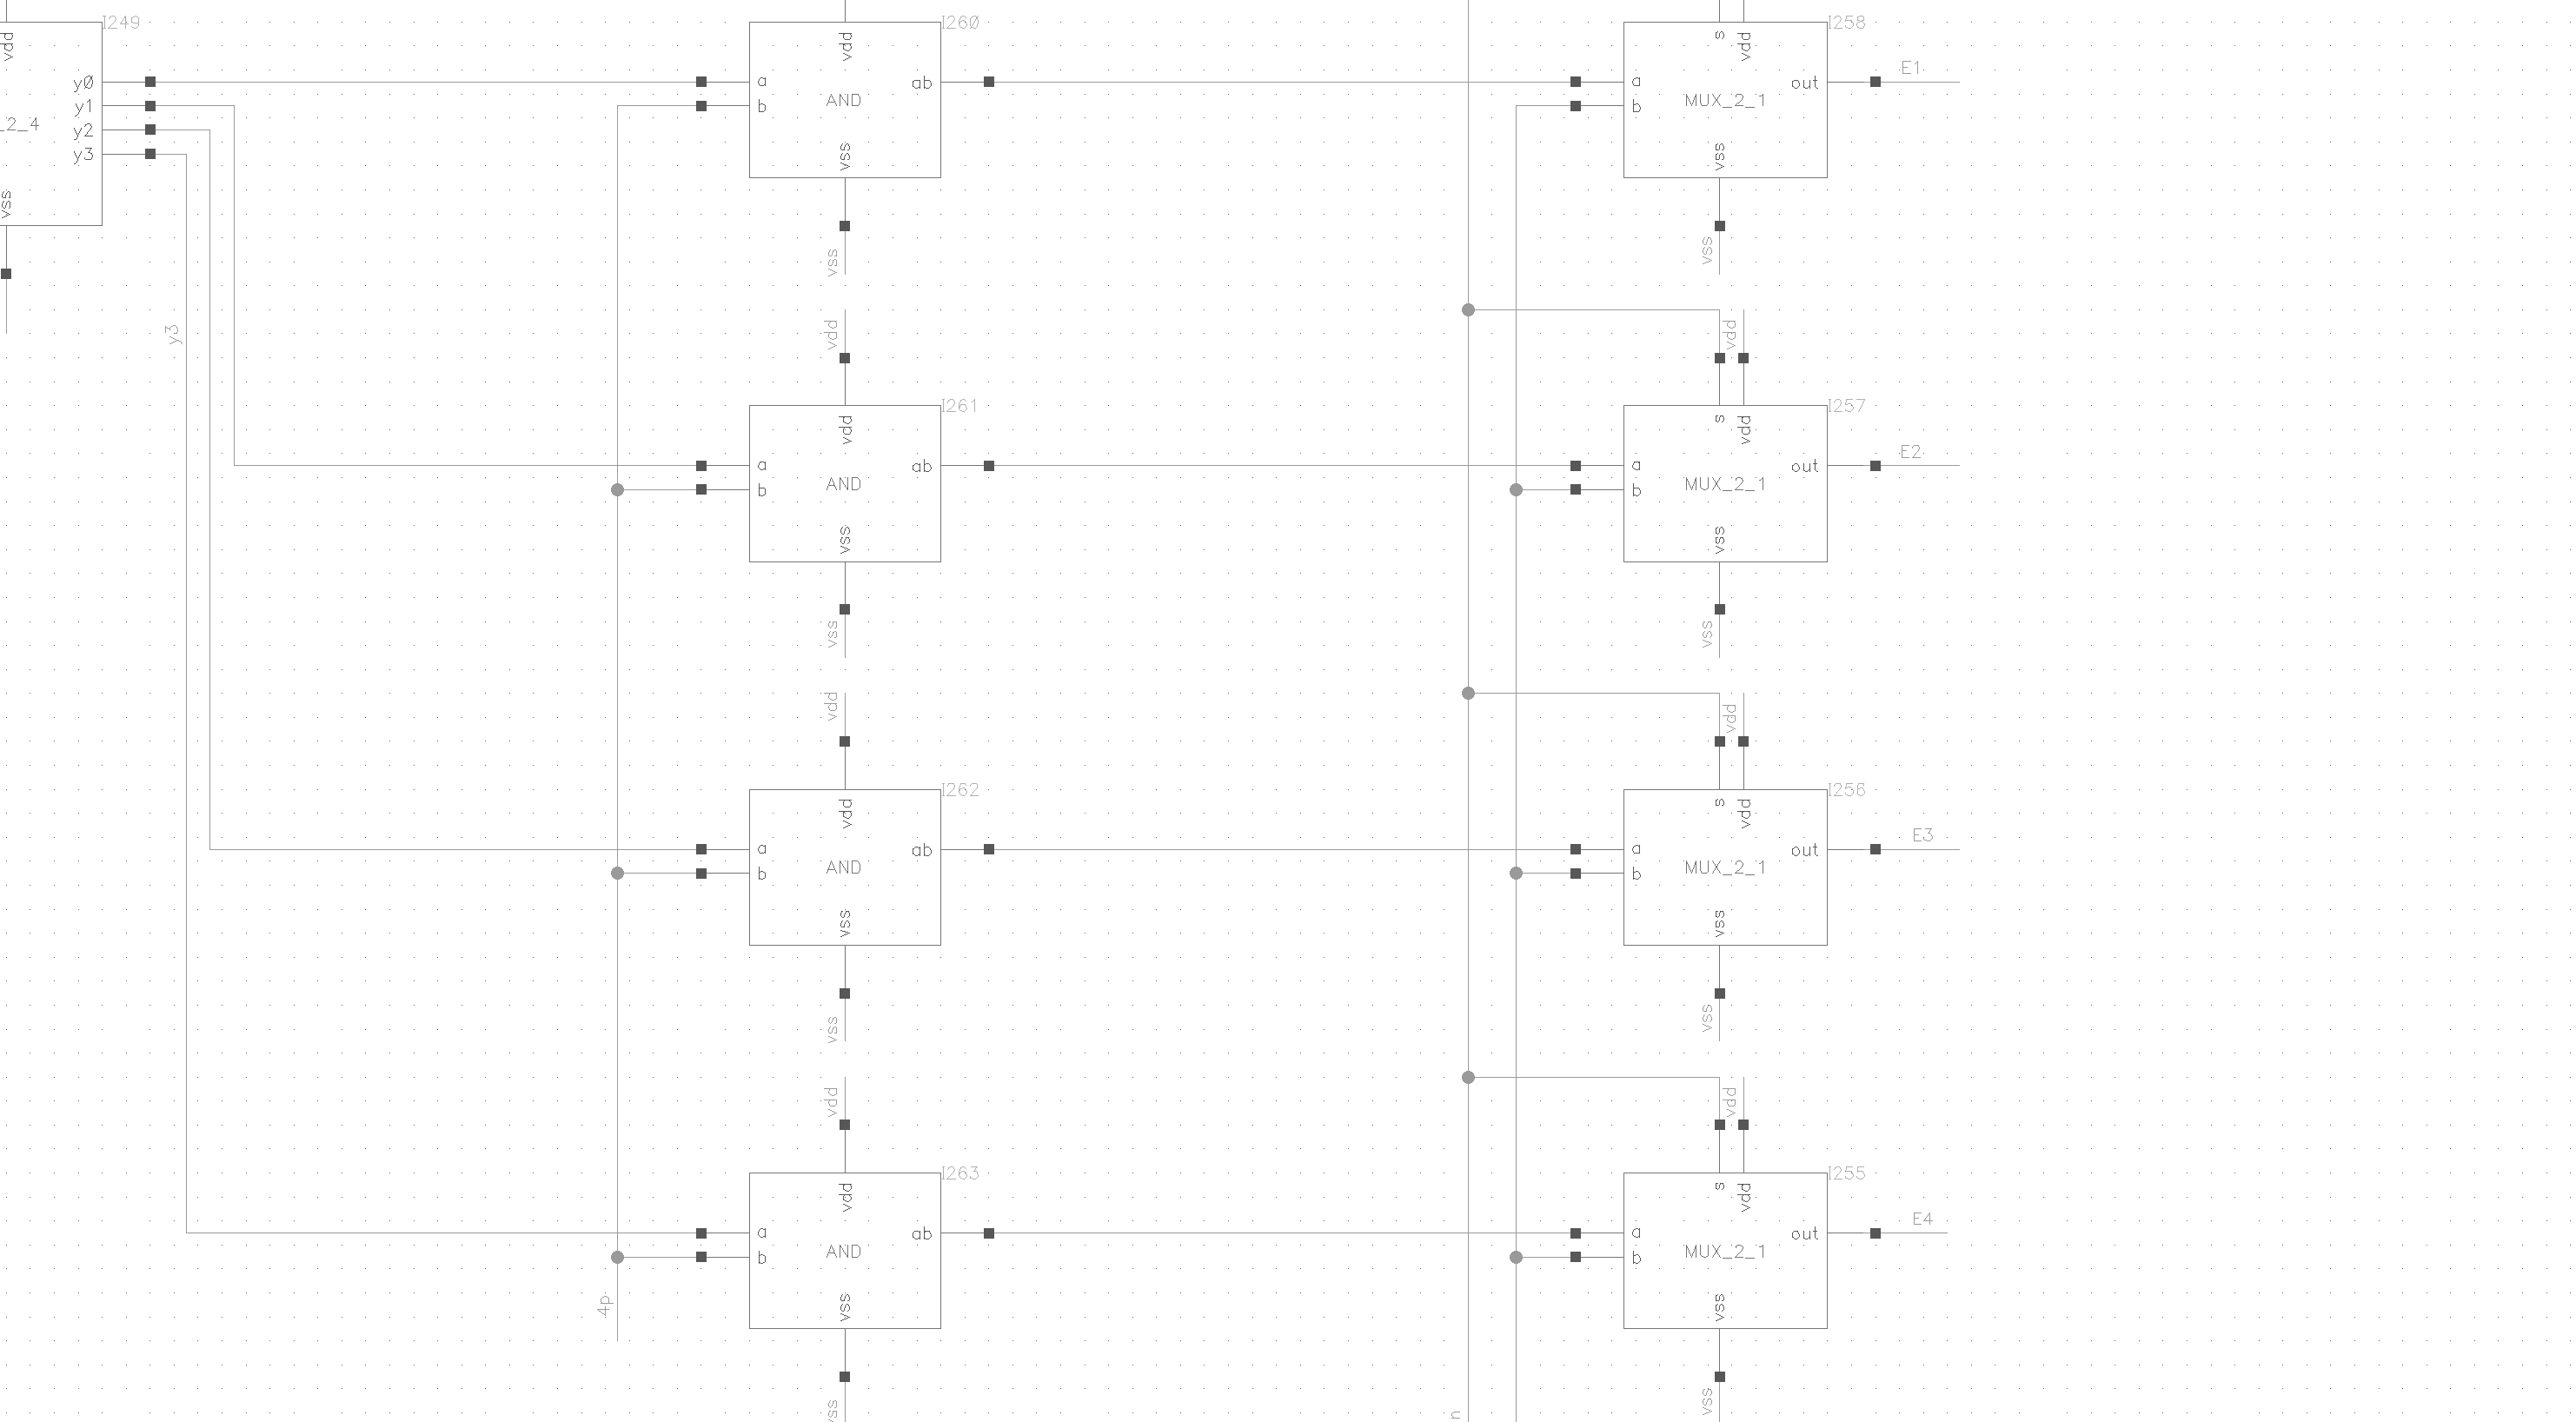
\includegraphics[scale=0.3]{../figures/spi_out2.png}
\caption{Control logic for spi output, second half}
\label{spi_out2}
\end{figure}

\subsection{Protocol}
This unit outputs the data with most significant bit first, in this case the carry output. To avoid using extra hardware, the group decided to go away from the more standard spi protocol.  \\
Data is both written and read by the chip on the rising edge of the the spi clock. This means that the circuitry communicating with the chip has to read and write on the falling edge of the clock. Additionally, the first bit of the output will be available on the second falling edge after spi enable goes low.

\subsection{Simulation results}
This section describes the resulting functionality of the system. The critical parts of the module are the events after a transition of the spi enable signal.
\subsubsection{High enable signal}
Figure \ref{sim_en_h} shows the simulation of the module when the spi enable signal goes high. As can be seen, the control logic successfully creates the four enable pulses for the different sections. The four clock cycles long pulse prevents the occurrence of more than one pulse on any of the enable signals. 


%\begin{figure}[H]
%\centering
%\captionsetup{justification=centering}
%\includegraphics[scale=0.2]{../figures/spi_en_high.png}
%\caption{Control logic for spi output, second half}
%\label{spi_en_h}
%\end{figure}


\subsubsection{Low enable signal}
Figure \ref{sim_en_l} shows that the enable signals are the same as the spi clock.

%\begin{figure}[H]
%\centering
%\captionsetup{justification=centering}
%\includegraphics[scale=0.2]{../figures/spi_out_low.png}
%\caption{Control logic for spi output, second half}
%\label{spi_en_l}
%\end{figure}


